\documentclass[pdf]{beamer}
%\documentclass[notes]{beamer}
%\documentclass{beamer}
\usepackage[utf8]{inputenc}
\usepackage{lmodern}
\usepackage{colortbl}
\usepackage{adjustbox}
%\usepackage{scrextend}
%\changefontsizes{7.5pt}

\usepackage{subfig}

\makeatletter
\makeatother
\usepackage{graphicx}

\mode<presentation>{\usetheme{Warsaw}}
%\mode<presentation>{\usetheme{Madrid}}
%% preamble
\title{Temas selectos de ciencia de datos}
\subtitle{Machine Translation para lenguajes con pocos recursos.}

\author{
Ricardo Cruz Sánchez \\
  \and
Rolando Corona Jiménez
}

\institute[CIMAT]{CIMAT}

\AtBeginSection[]{%
\begin{frame}
    \tableofcontents[currentsection, subsectionstyle=show/show/hide]
\end{frame}
}

\begin{document}

\begin{frame}
\titlepage
\end{frame}

%\AtBeginSubsection[]
%{
%  \begin{frame}<beamer>
%    \frametitle{Contenido}
%    \tableofcontents[currentsection,currentsubsection]
%  \end{frame}
%}



\section{Introducción}

\begin{thebibliography}{1}

\bibitem{cr98}
Lorrie Faith Cranor and Brian A. LaMacchia. 1998. Spam!. Commun. ACM 41, 8 (August 1998), 74-83. 

\bibitem{fe19}
Emilio Ferrara. 2019. The history of digital spam. Commun. ACM 62, 8 (July 2019), 82-91. 

\bibitem{ha01}
Hastie, T., Tibshirani, R.,, Friedman, J. (2001). The Elements of Statistical Learning. New York, NY, USA: Springer New York Inc.. 

\bibitem{so09}
Marina Sokolova and Guy Lapalme. 2009. A systematic analysis of performance measures for classification tasks. Inf. Process. Manage. 45, 4 (July 2009), 427-437. 

\end{thebibliography}



\end{document}























\section{Modelos de clasificación.}
\begin{frame}{Segmentación de la muestra}
\begin{itemize}
\item muestreo aleatorio para generar ambas submuestras. El conjunto de entrenamiento consiste de 3680 observaciones (aproximadamente un $80\%$) y el de prueba contiene 921 observaciones.
\end{itemize}
\end{frame}


\begin{frame}{Logistica}
\begin{itemize}
\item  Su característica principal es el tener una variable dependiente dicotómica. Utilizá la función enlace \emph{logit} y gracias a esto se modela:

$$logit(p)=ln(\dfrac{p}{1-p})=\beta x$$

donde $p$ corresponde a la probabilidad asociada a la distribución binomial de la cual se generan los valores de $y$, es decir, $y\thicksim Bin(n,p)$\\


\end{itemize}
\end{frame}


\begin{frame}{Logistica}
\begin{itemize}
\item  Una vez que se encuentran los parámetros $\beta$, solo es cuestión de evaluar la observación de las variables independientes $x$ y obtener el valor de $p$ aplicando la función inversa de \emph{logit}.\\

\item El valor estimado de $y$ dependerá de $p$ y un \emph{punto de corte}, que usualmente es el valor $0.5$, ya que si la observación es más grande que el punto de corte quiere decir que $y$ se asemeja más a la distribución de los valores $y=1$ y se asignará como 1. En caso de ser menor al punto de corte se determina que el valor estimado es 0.\\
\end{itemize}
\end{frame}


\begin{frame}{Logistica}
\begin{figure}
\centering
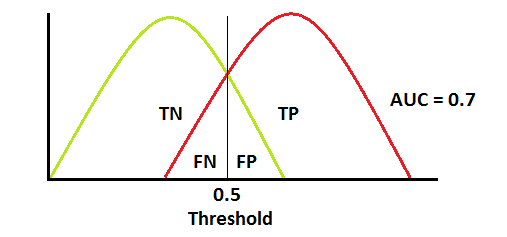
\includegraphics[scale=.75]{images/punto_de_corte.png} 
\caption{Distribuciones de TP y FP con relación al punto de corte.}
\label{cutoff}
\end{figure}
\end{frame}


\begin{frame}{Logistica full}
\begin{figure}[h]
 \centering
  \subfloat[Entrenamiento]{
    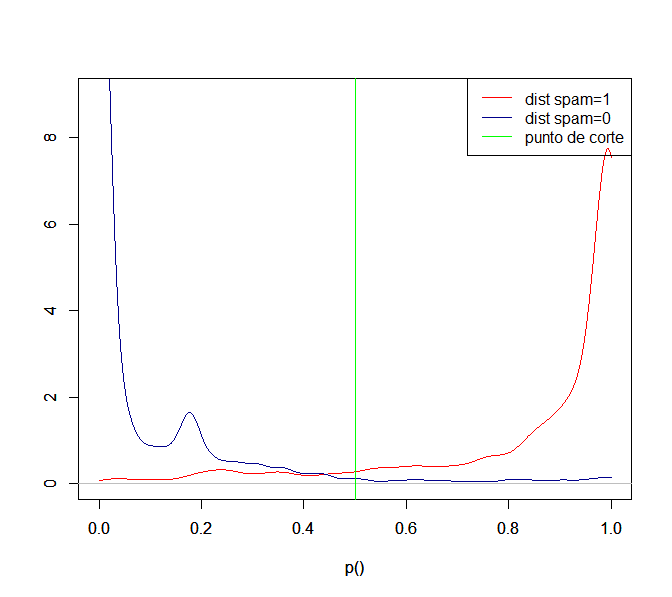
\includegraphics[width=0.5\textwidth]{images/dist1.png}}
  \subfloat[Prueba]{
    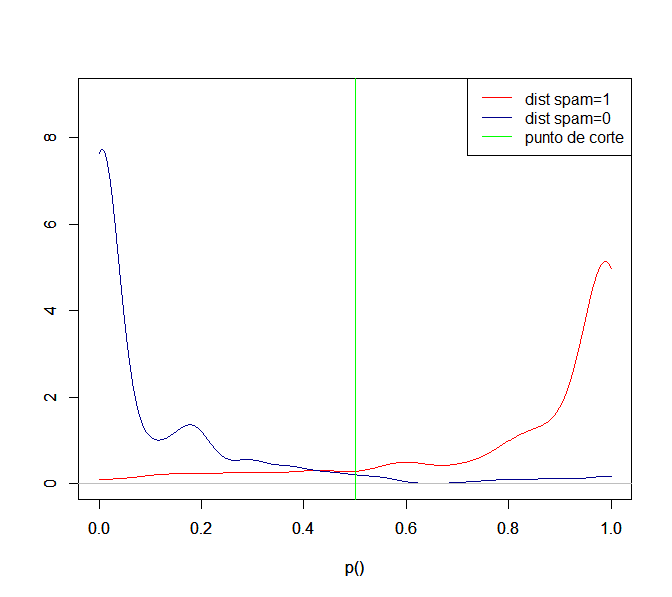
\includegraphics[width=0.5\textwidth]{images/dist2.png}}
 \caption{Densidades TP y TN}
 \label{log2}
\end{figure}
\end{frame}


\begin{frame}{Logistica full}
\begin{table}[ht]
\centering
\begin{tabular}{|l|l|l|}
\hline
&Entrenamiento&Prueba\\
\hline\hline
Accuracy& $.93$ & $.92 \%$ \\ \hline
Recall & $.90$ & $.88 \%$ \\ \hline
Specificity & $.92$ & $.94 \%$ \\ \hline
\end{tabular}
\caption{Métricas modelo full.}
\label{log1}
\end{table}
\end{frame}




\begin{frame}{Logistica cutoff}
\begin{figure}[h]
 \centering
  \subfloat[Entrenamiento]{
    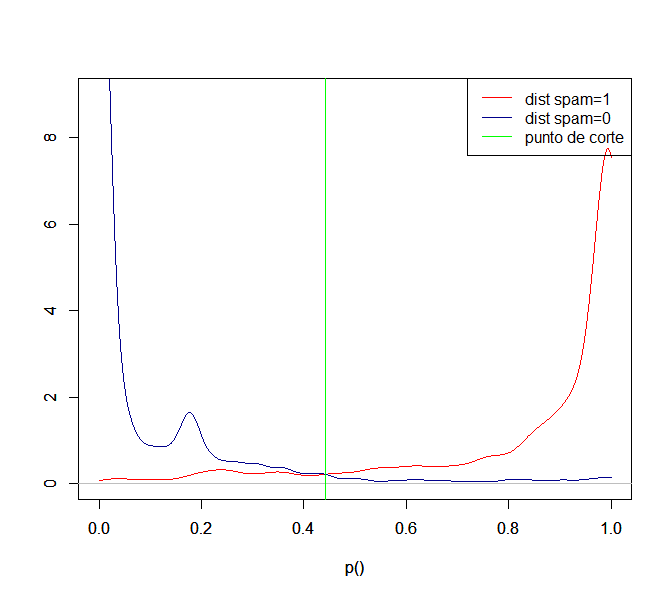
\includegraphics[width=0.5\textwidth]{images/dist3.png}}
  \subfloat[Prueba]{
    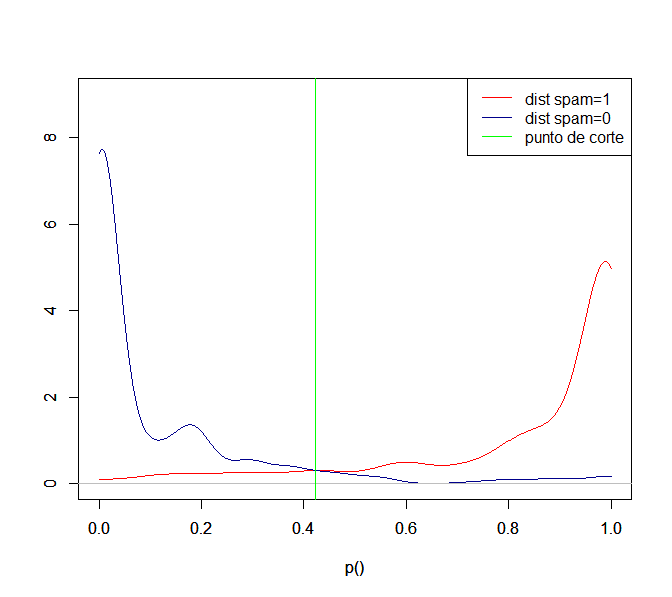
\includegraphics[width=0.5\textwidth]{images/dist4.png}}
 \caption{Densidades TP y TN}
 \label{log4}
\end{figure}
\end{frame}



\begin{frame}{Logistica cutoff}
\begin{table}[ht]
\centering
\begin{tabular}{|l|l|l|}
\hline
&Entrenamiento&Prueba\\
\hline\hline
Accuracy& $.93\%$ & $.91 \%$ \\ \hline
Recall & $.91\%$ & $.90 \%$ \\ \hline
Specificity & $.95\%$ & $.93 \%$ \\ \hline
\end{tabular}
\caption{Métricas modelo full, punto de corte 0.42}
\label{log3}
\end{table}
\end{frame}

\begin{frame}{Logistica zero false positives}
si la estrategia a seguir fuese no dejar pasar como spam a ningún correo que realmente no sea spam, entonces el punto de corte debe despalzarse hasta la probabilidad máxima observada en los verdaderos negativos durante el entrenamiento.
\end{frame}

\begin{frame}{Logistica zero false positives}
\begin{table}[ht]
\centering
\begin{tabular}{|l|l|l|}
\hline
&Entrenamiento&Prueba\\
\hline\hline
Accuracy& $.63\%$ & $.63 \%$ \\ \hline
Recall & $.08\%$ & $.09 \%$ \\ \hline
Specificity & $1\%$ & $1 \%$ \\ \hline
\end{tabular}
\caption{Métricas modelo full, punto de corte 0.9945}
\label{log5}
\end{table}
\end{frame}

\begin{frame}{separación completa}
\begin{itemize}
\item En las densidades mostradas se puede observar que las distribuciones se concentran demasiado en los extremos, es decir, las probabilidades generadas están muy cerca de 0 y 1. De hecho, esto aparece como un \emph{warning} al generar los modelos, en consola se puede leer que se generaron probabilidades 0 ó 1.\\

\item Este comportamiento se conoce como \emph{separación completa o quasi completa} y se genera cuando para una categoría en particular, se puede observar el valor constante de alguna o algunas variables, lo cual llevaría a que se pueda determinar el valor de la respuesta con solo ver las variables que son constantes, es decir, sería un modelo determinista.\\

\end{itemize}
\end{frame}

\begin{frame}{separación completa, selección}
\begin{figure}[h]
 \centering
  \subfloat[Entrenamiento]{
    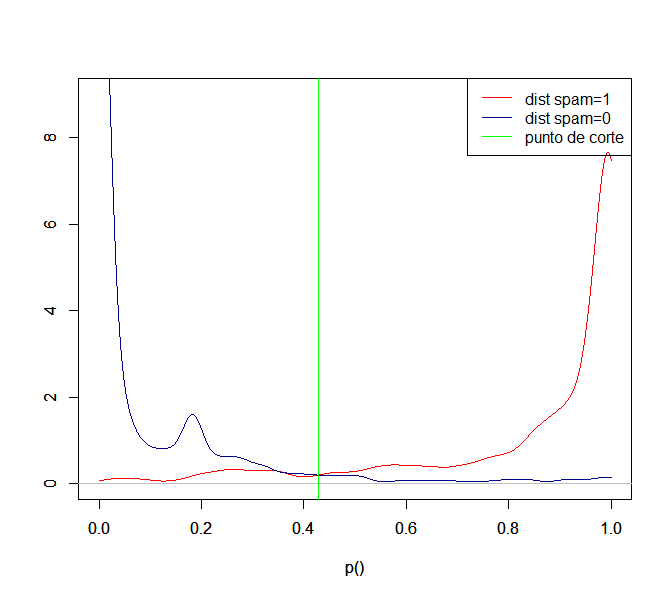
\includegraphics[width=0.5\textwidth]{images/dist5.png}}
  \subfloat[Prueba]{
    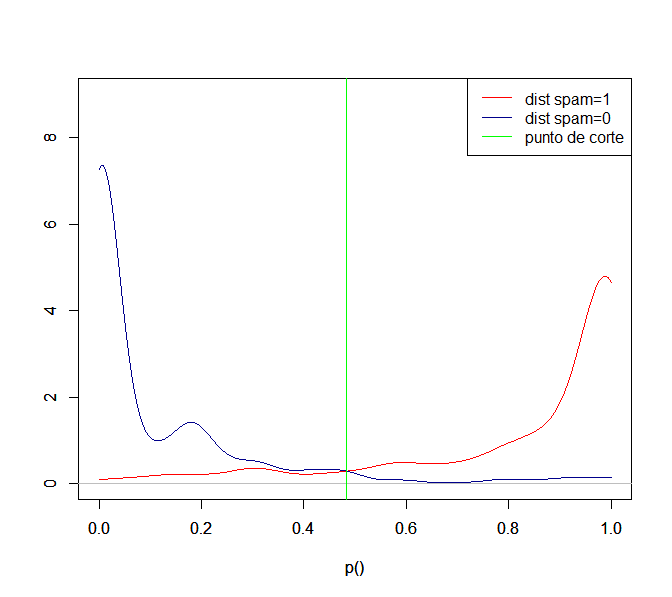
\includegraphics[width=0.5\textwidth]{images/dist6.png}}
 \caption{Densidades TP y TN}
 \label{log7}
\end{figure}
\end{frame}

\begin{frame}{separación completa, selección}
\begin{table}[ht]
\centering
\begin{tabular}{|l|l|l|}
\hline
&Entrenamiento&Prueba\\
\hline\hline
Accuracy& $.93\%$ & $.92 \%$ \\ \hline
Recall & $.91\%$ & $.88 \%$ \\ \hline
Specificity & $.94\%$ & $.94 \%$ \\ \hline
\end{tabular}
\caption{Métricas modelo stepwisw}
\label{log6}
\end{table}
\end{frame}


\begin{frame}{coeficientes}
Finalmente, en este método, se consideraron los coeficientes más importantes de acuerdo a la magnitud que poseían:

\begin{itemize}
\item char$\_$freq$\_\$$: 6.66
\item cs: -508.4
\item george: -9.81
\item conference: -4.52
\item meeting: -2.69
\end{itemize} 

\end{frame}


\begin{frame}{Regularización}
\begin{itemize}

\item Una de las posibles alternativas son los métodos de regularización, los cuales pueden seleccionar variables y mejorar las estimaciones de los coeficientes haciendolos tender a 0.\\

\item Para implementar estos dos métodos, primero se realiza validación cruzada, con lo que se determinará el valor de $\lambda$ en cada caso. \\

\end{itemize}
\end{frame}


\begin{frame}{Regularización}
\begin{figure}[h]
 \centering
  \subfloat[Entrenamiento]{
    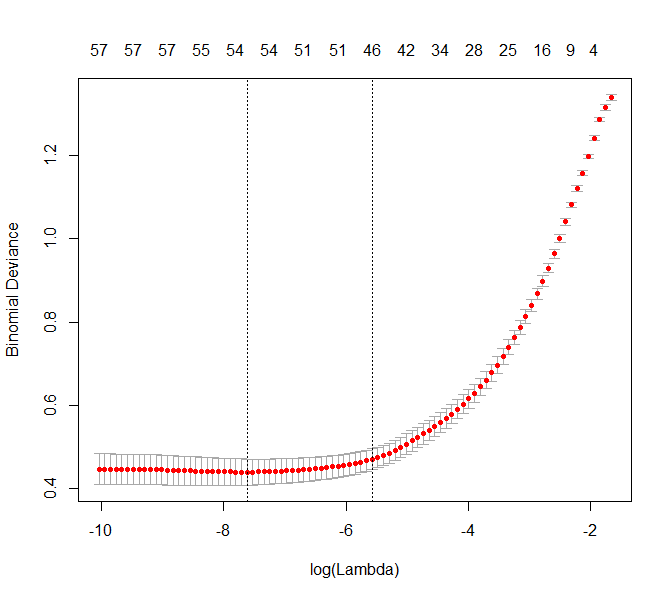
\includegraphics[width=0.5\textwidth]{images/scree1.png}}
  \subfloat[Prueba]{
    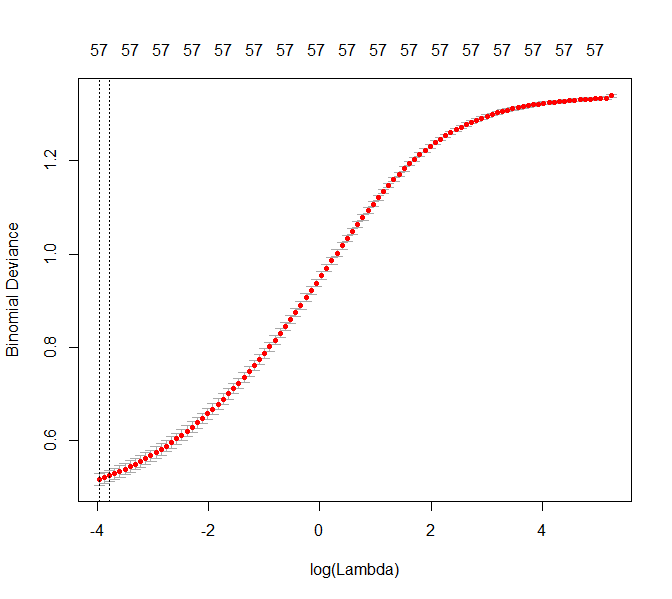
\includegraphics[width=0.5\textwidth]{images/scree2.png}}
 \caption{Densidades TP y TN}
 \label{screeplots}
\end{figure}
\end{frame}

\begin{frame}{Regularización}
C-V sugiere utilizar $\lambda=.018$ para ridge y $\lambda=0.00049$ para lasso. Con estos dos valores lasso selecciona 54 variables, mientras que ridge ocupa todas aunque las aproxima a 0.\\
\end{frame}

\begin{frame}{Regularización}
\begin{table}[ht]
\centering
\begin{tabular}{|l|l|l|}
\hline
&Lasso&Ridge\\
\hline\hline
Accuracy& $.90\%$ & $.87 \%$ \\ \hline
Recall & $.82\%$ & $.73 \%$ \\ \hline
Specificity & $.96\%$ & $.96 \%$ \\ \hline
\end{tabular}
\caption{Métricas modelo lasso y ridge}
\label{lasso}
\end{table}
\end{frame}

\begin{frame}{svm y regresión bayesiana}
\begin{table}[ht]
\centering
\begin{tabular}{|l|l|l|}
\hline
&SVM&Bayes\\
\hline\hline
Accuracy& $.91\%$ & $.91 \%$ \\ \hline
Recall & $.88\%$ & $.91 \%$ \\ \hline
Specificity & $.93\%$ & $.92 \%$ \\ \hline
\end{tabular}
\caption{Métricas svm y regresion bayesiana}
\label{svm}
\end{table}\end{frame}


